%\chapter{Obsah CD}
%\chapter{Manual}
%\chapter{Konfigra�n� soubor}
%\chapter{RelaxNG Sch�ma konfigura�n�ho soboru}
%\chapter{Plakat}

\chapter{Diagram HTML 5 API}
\label{priloha:html5}
\begin{figure}[htb]
\centering
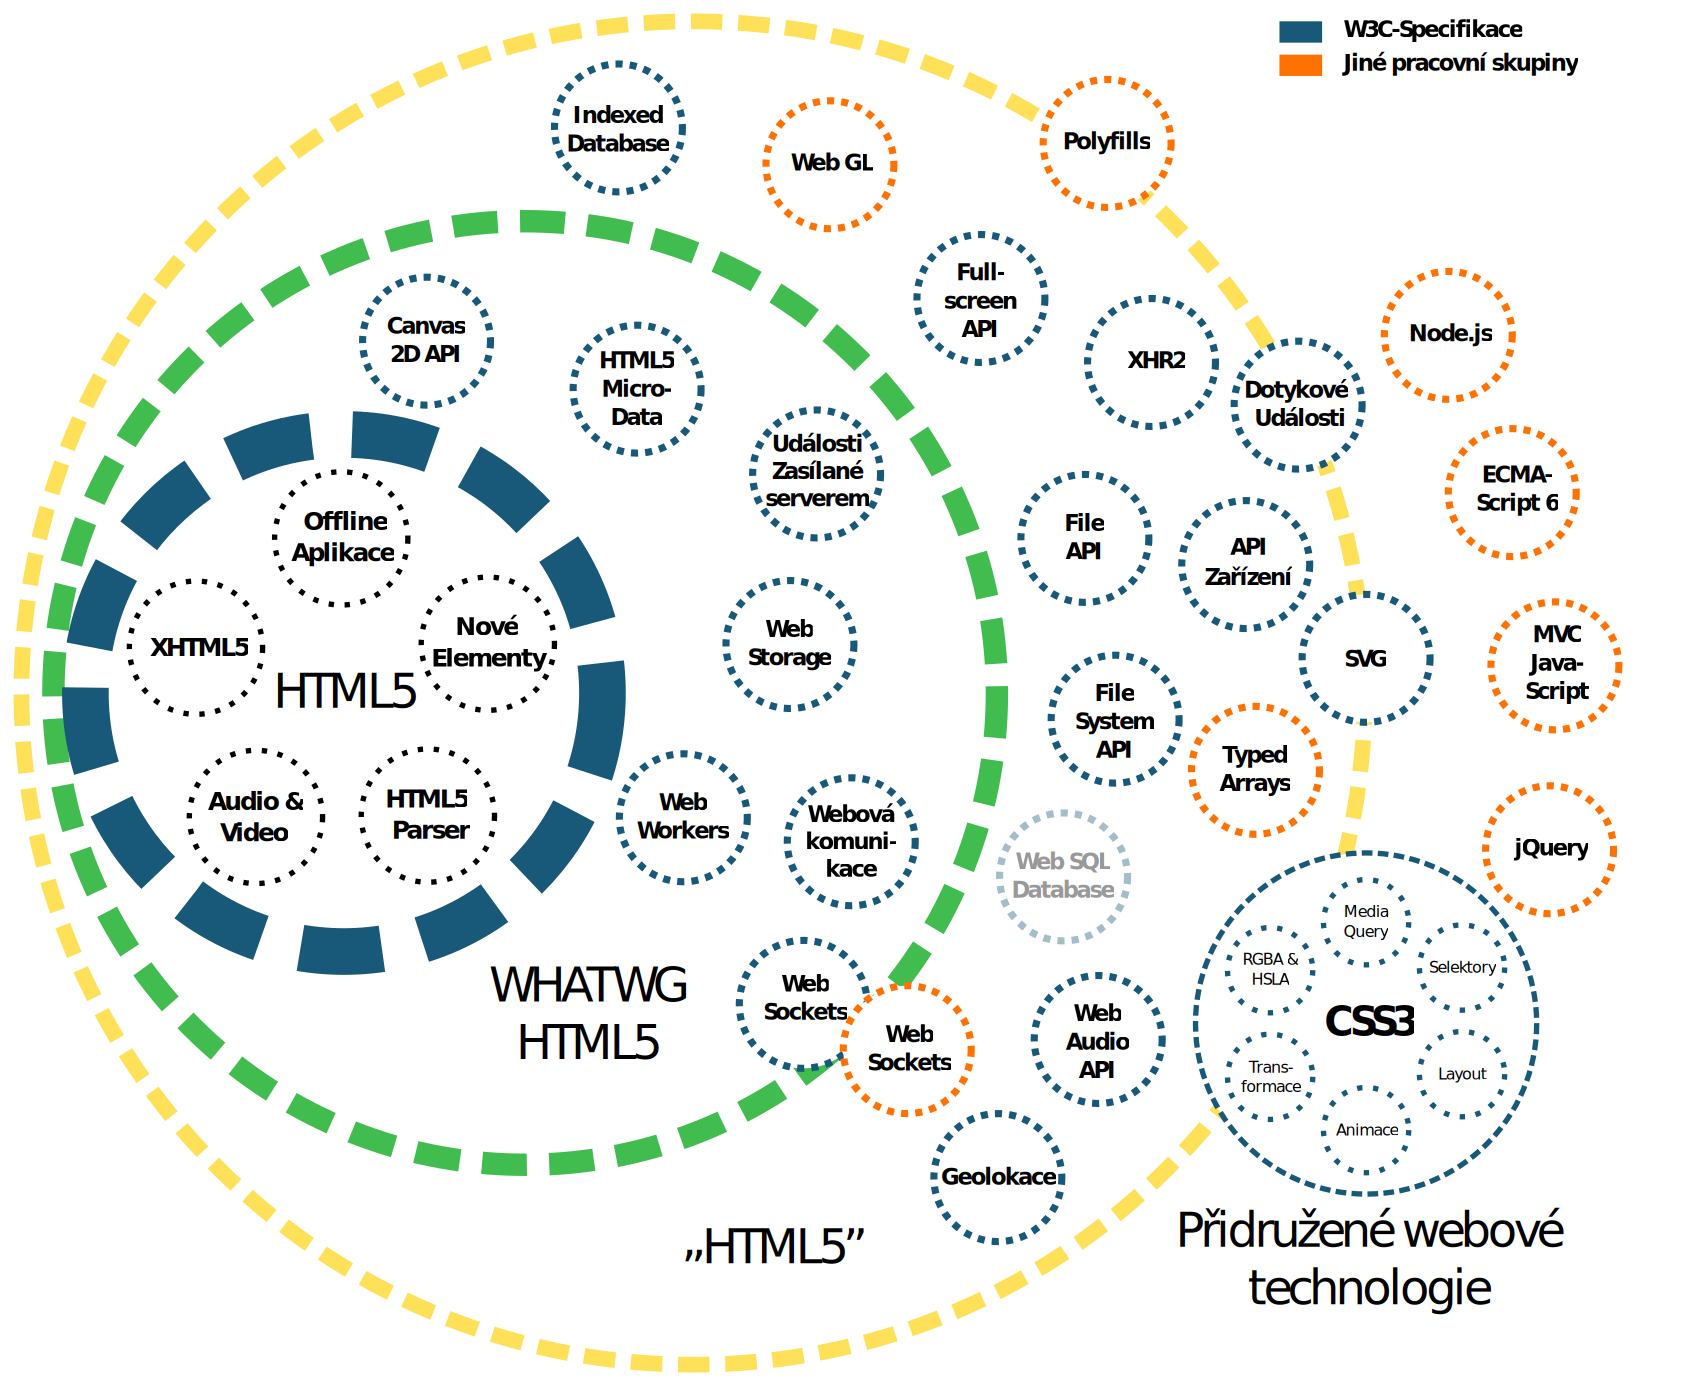
\includegraphics[width=1.0\textwidth]{html5api}
\caption{HTML 5 API}
\label{fig:html5api}
\end{figure}

\chapter{Diagram n�vrhu webu}
\begin{figure}[htb]
\centering
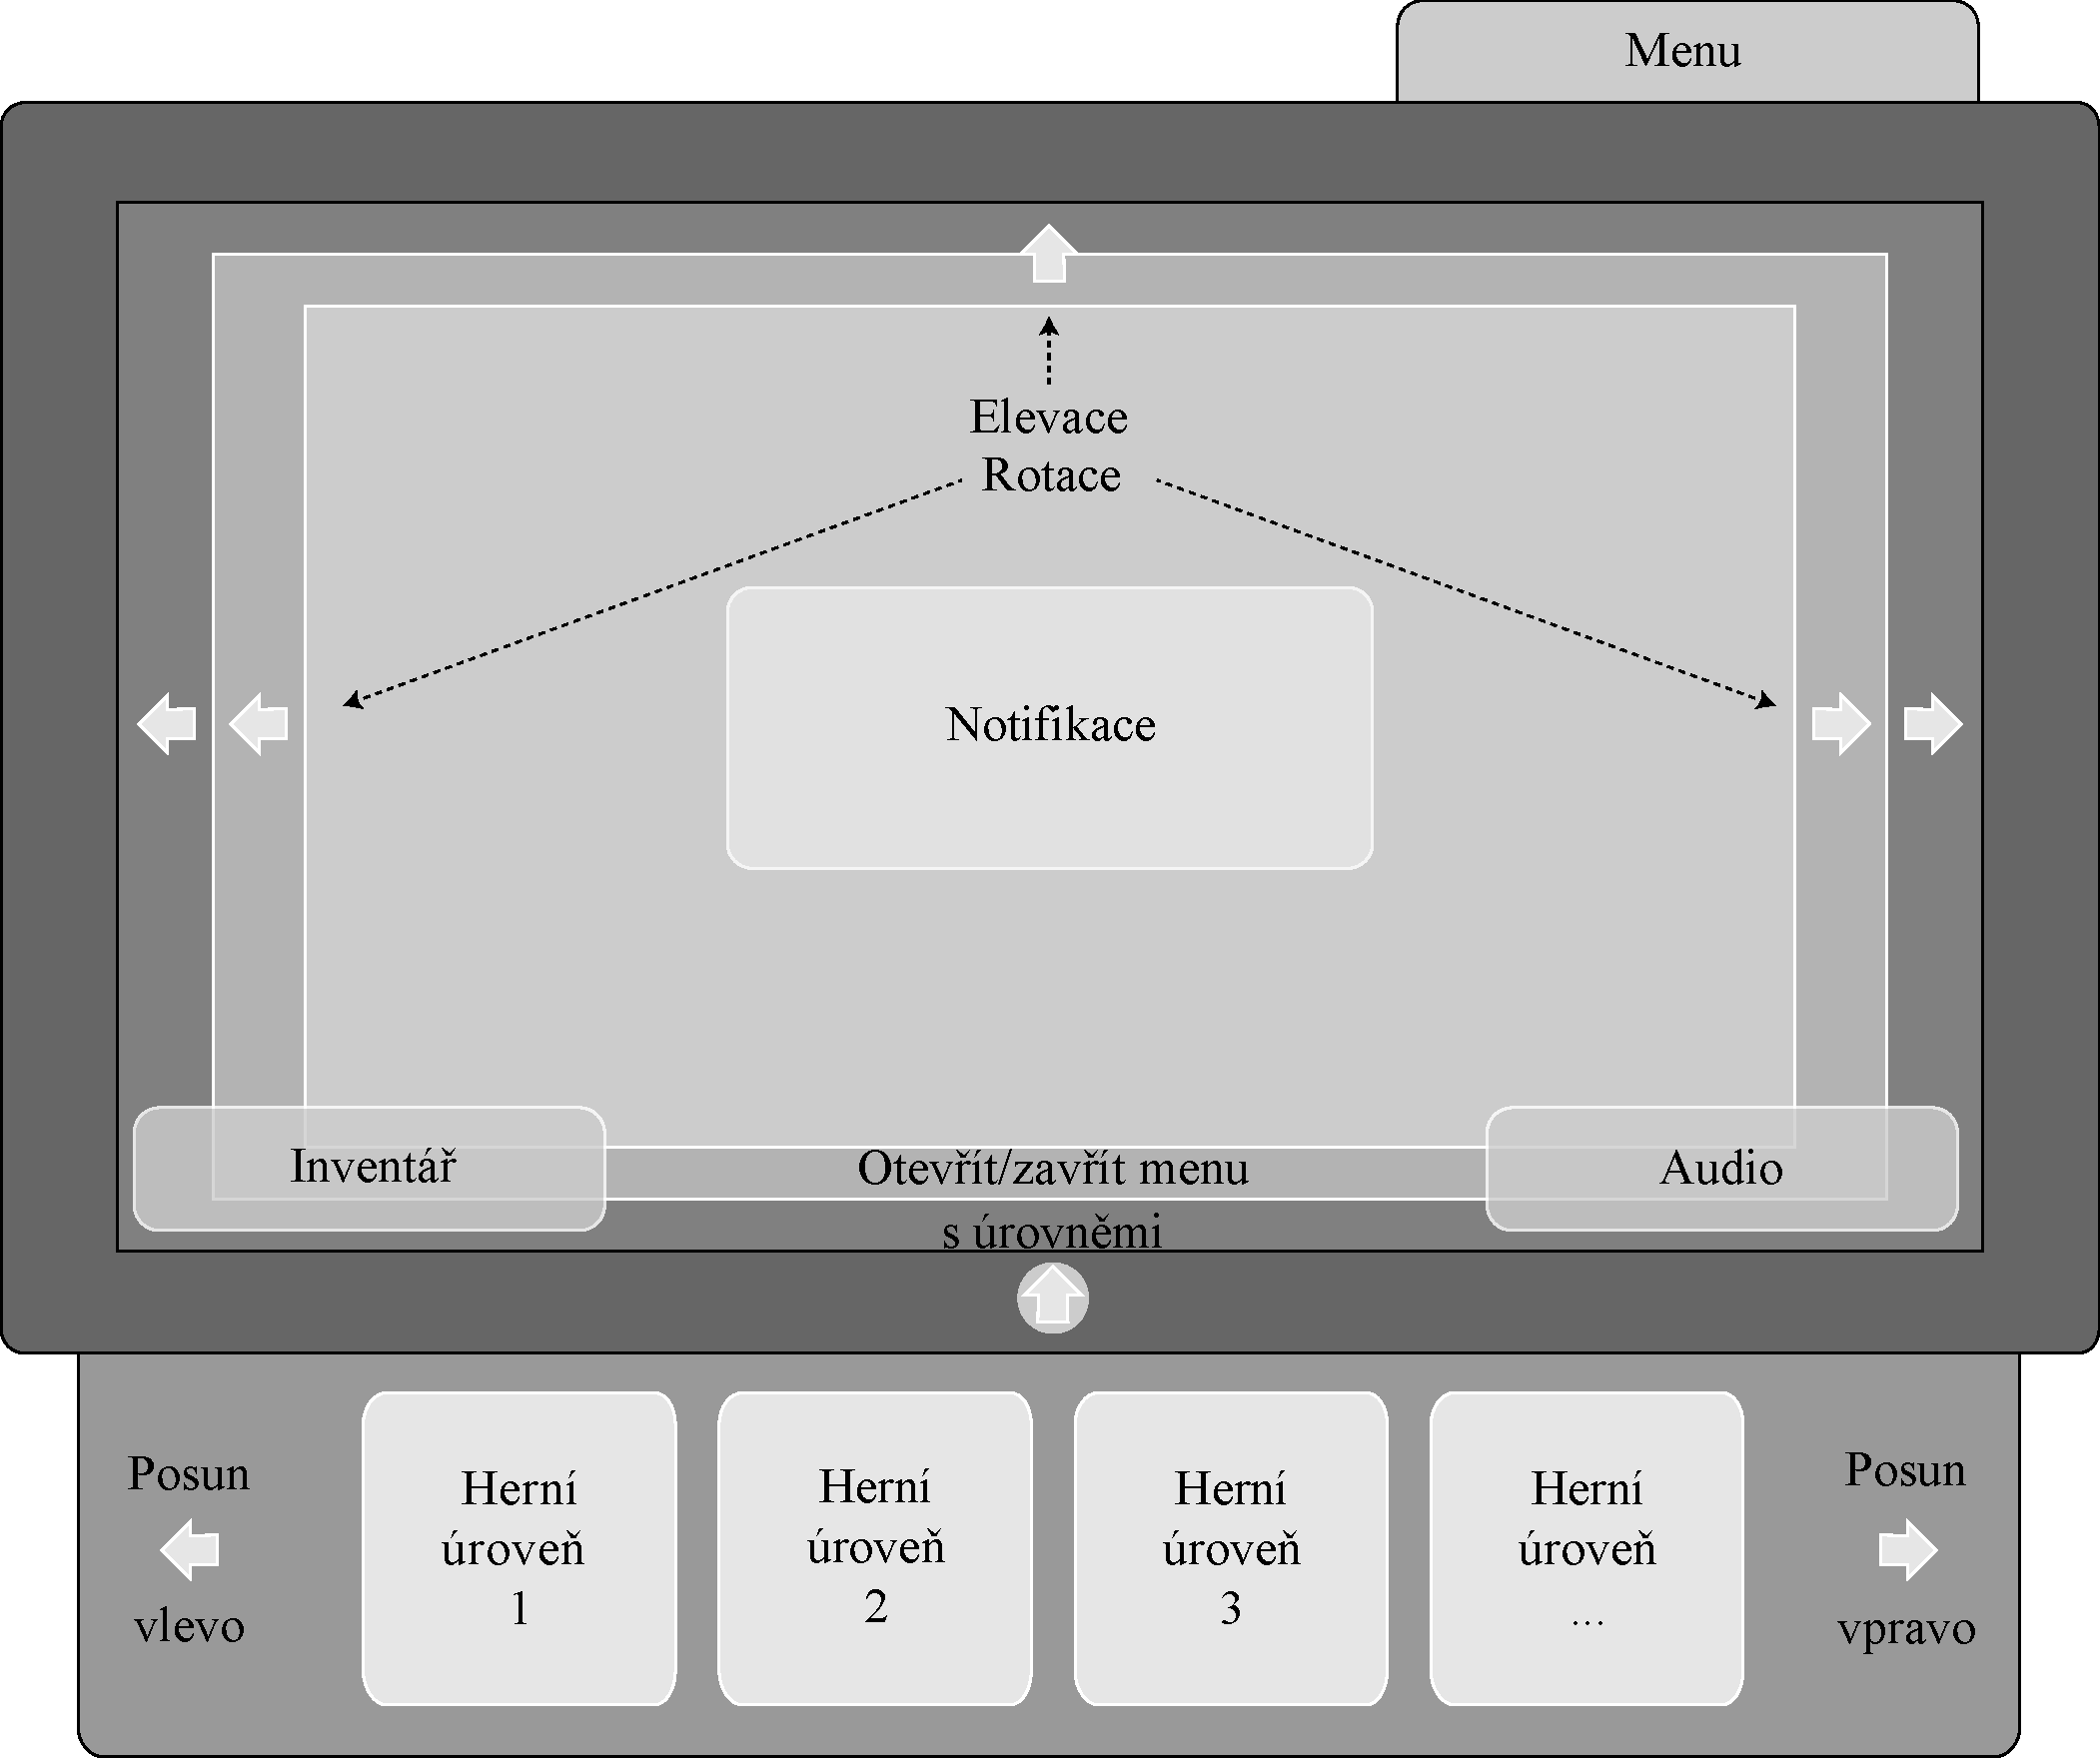
\includegraphics[width=1.0\textwidth]{web}
\caption{N�vrh webu}
\label{fig:web}
\end{figure}

%\chapter{Diagram ovl�d�n� kamery}
%\begin{figure}[htb]
%\centering
%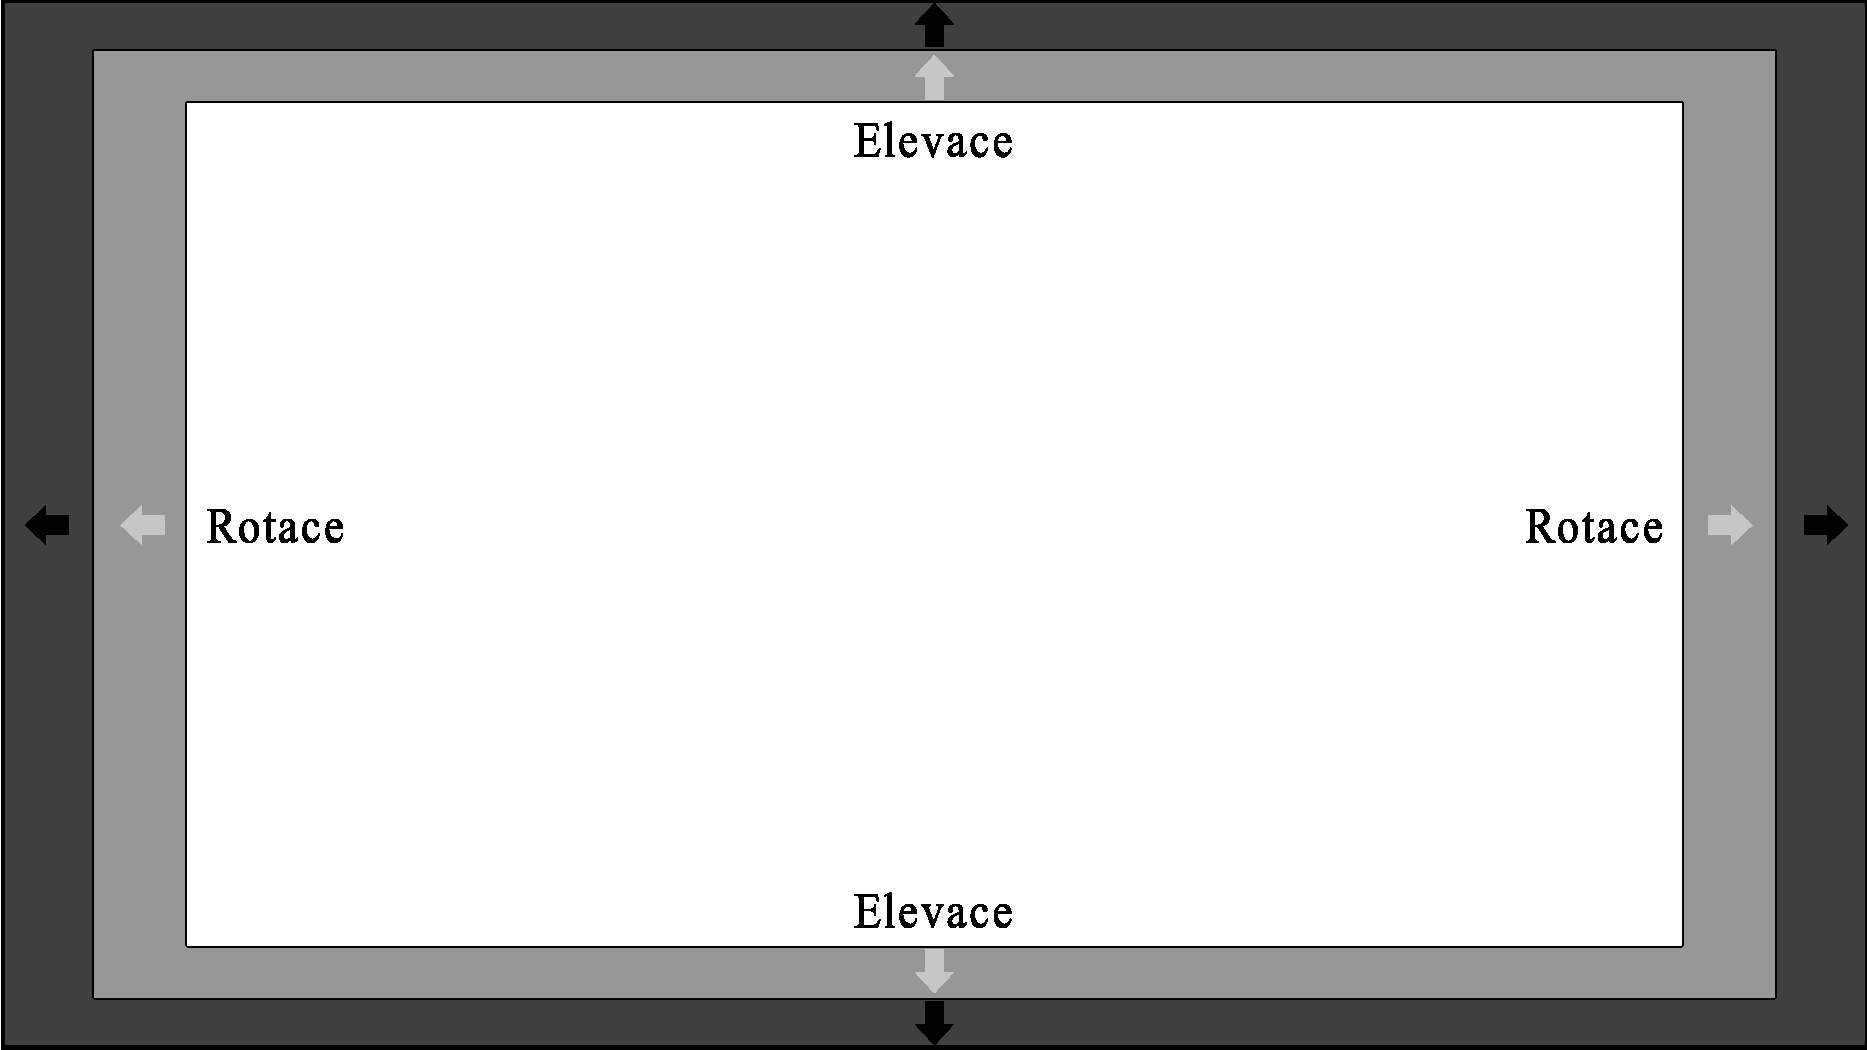
\includegraphics[width=1.0\textwidth]{mouseCamera}
%\caption{Ovl�d�n� kamery}
%\label{fig:mouseCamera}
%\end{figure}

\chapter{Podoba hry Beru�ky 2 WebGL}
\begin{figure}[htb]
\centering
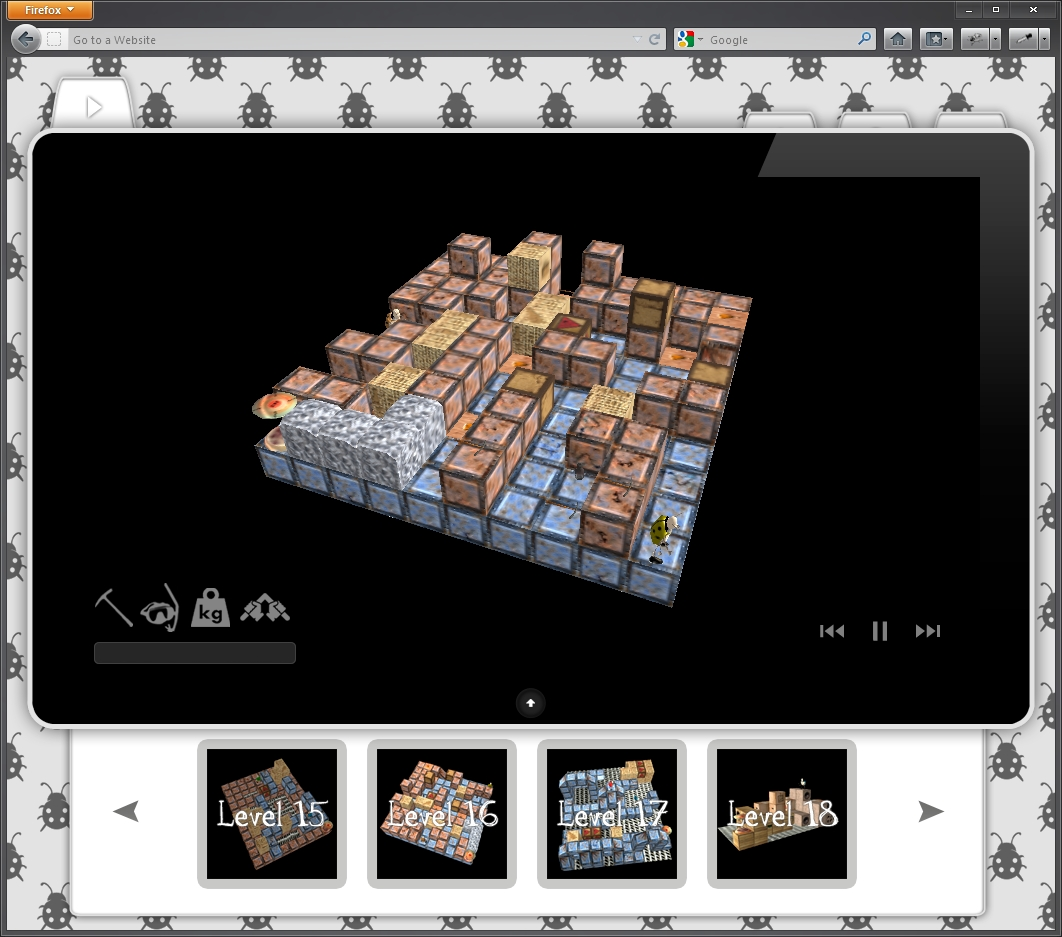
\includegraphics[width=1.0\textwidth]{bugEscapeWebGL}
\caption{Beru�ky 2 WebGL v prohl��e�i Firefox 12}
\label{fig:gameImage}
\end{figure}

\chapter{Obsah DVD}
\begin{table}[!ht]
\label{table:dvd}
\begin{center}
\begin{tabular}{ | l | l |}
\hline
\textbf{Cesta} & \textbf{Popis} \\ \hline
\texttt{./audio} & Hern� hudba \\ \hline
\texttt{./css} & Kask�dov� styly \\ \hline
\texttt{./doc} & Zdrojov� soubory t�to pr�ce \\ \hline
\texttt{./dochtml} & Vygenerovan� HTML dokumentace \\ \hline
\texttt{./graphics} & Zdrojov� soubory grafiky \\ \hline
\texttt{./img} & Webov� grafika \\ \hline
\texttt{./js} & Implementace hry a soubory framework� \\ \hline
\texttt{./levels} & JSON soubory hern�ch �rovn� \\ \hline
\texttt{./lightmaps} & Lightmapy \\ \hline
\texttt{./textures} & Textury \\ \hline
\textbf{\texttt{./index.html}} & HTML dokument hry s GLSL popisem shader� \\ \hline
\end{tabular}
\end{center}
\caption{Obsah DVD}
\end{table}



